\section{Алгоритм Extended Position Based Dynamics} \label{ch2:xpbd} %название по-русски
	В статье \cite{muller2020detailed} авторами оригинальной статьи Position Based Dynamics были обозначены шесть основных проблем данного алгоритма:
	\begin{enumerate}[1.]
		\item Числа, использующиеся в качестве параметров, не являются физическими величинами.
		\item Жесткость симулируемого мягкого тела зависит как от количества итераций, так и от величины временного шага.
		\item Интегрирование не является физически точным.
		\item Результат зависит от порядка.
		\item Результат зависит от геометрической структуры ткани.
		\item Алгоритм медленно сходится.
	\end{enumerate}
	
	Для решения первых трех проблем авторами был разработан алгоритм Extended Position Based Dynamics \cite{xpbd}, являющийся улучшением оригинального. Для этого авторы взяли известное уравнение
	\begin{equation}
		\textbf{M}\ddot{x} = -\nabla U^T(x)
	\end{equation}
	
	В данном уравнении под $\textbf{M}$ понимаются матрица с массами частиц, под $x$ вектор из положений частиц, а под $U$ - потенциальная энергия частиц. Если дискретизировать данное уравнение по времени, то мы получим следующее уравнение:
	\begin{equation}
		\textbf{M}(\frac{x^{n+1} - 2x^n + x^{n-1}}{\Delta t^2}) = -\nabla U^T(x^{n+1})
	\end{equation}
	
	Записав потенциальную энергию через функции ограничения, описанные в \cite{servin2006interactive}, мы получаем систему уравнений:
	\begin{equation} \label{eq:xpbd_first}
		\textbf{M}(x^{n+1} - 2x^n + x^{n-1}) - \nabla \textbf{C}(x^{n+1})^T\lambda^{n+1} = 0
	\end{equation}
	\begin{equation} \label{eq:xpbd_second}
		\textbf{C}(x^{n+1}) + \frac{\alpha}{\Delta t^2}\lambda^{n+1} = 0		
	\end{equation}
	
	В данной системе $\textbf{C} = [C_1(x), C_2(x),... C_M(x)]^T$ - вектор, состоящий из функций ограничения, $\lambda = [\lambda_1, \lambda_2, ..., \lambda_M]^T$ - вектор множителей ограничений, $\alpha$ - диагональная матрица содержащая значения, обратные величине жесткости каждого ограничения. Если мы обозначим выражение \ref{eq:xpbd_first} как $g(x, \lambda) = 0$, а выражение \ref{eq:xpbd_second} как $h(x, \lambda) = 0$, то, воспользовавшись методом Ньютона для решения полученной системы, мы получаем систему вида:

\begin{equation}
	\left[
		\begin{array}{cc}
			\frac{\delta g}{\delta x} & -\nabla \textbf{C}^T(x_i)\\
			\nabla \textbf{C}(x_i) & \frac{\alpha}{\Delta t^2}
		\end{array}
	\right]\left[
		\begin{array} {c}
			\Delta x\\
			\Delta \lambda
		\end{array}
	\right]	= -\left[
		\begin{array}{c}
			g(x_i, \lambda_i)\\
			h(x_i, \lambda_i)
		\end{array}
	\right]
\end{equation}

	Далее, авторы статьи вносят два допущения. Первое - принимается что $\frac{\delta g}{\delta x} = M$. Это исключает геометрическую жесткость и вносит погрешность порядка $O(\Delta t^2)$ (данный метод тогда можно рассматривать как квази-Ньютоновский). Второе - $g(x_i, \lambda_i) = 0$. Хотя это верно только для первой итерации метода Ньютона (при $x_0 = 2x^n + x^{n-1}$, $\lambda_0 = 0$), если $\nabla \textbf{C}^T$ будет изменяться медленно, то значение $g(x_i, \lambda_i)$ будет отставаться малым, и станет равно нулю, когда $\nabla \textbf{C}^T$ станет константным. Если внести эти две аппроксимации, то система \ref{eq:xpbd-system-hard} будет иметь вид:
\begin{equation} \label{eq:xpbd-system-hard}
	\left[
	\begin{array}{cc}
		\textbf{M} & -\nabla \textbf{C}^T(x_i)\\
		\nabla \textbf{C}(x_i) & \frac{\alpha}{\Delta t^2}
	\end{array}
	\right]\left[
	\begin{array} {c}
		\Delta x\\
		\Delta \lambda
	\end{array}
	\right]	= -\left[
	\begin{array}{c}
		0\\
		h(x_i, \lambda_i)
	\end{array}
	\right]
\end{equation}

	Взяв дополнение Шура \cite{prasolov1996} мы можем получить следующую систему относительно $\Delta \lambda$:
\begin{equation} \label{eq:xpbd-delta-lambda}
	\left[\nabla \textbf{C}(x_i) \textbf{M}^{-1} \nabla \textbf{C}^T(x_i) + \frac{\alpha}{\Delta t^2}\right]\Delta \lambda = -\textbf{C}(x_i) - \frac{\alpha}{\Delta t^2}\lambda_i
\end{equation}	

	Значение $\Delta x$ может быть высчитано с помощью следующего выражения:
\begin{equation} \label{eq:xpbd-delta-x}
	 \Delta x = \textbf{M}^{-1} \nabla \textbf{C}^T(x_i) \Delta \lambda
\end{equation}	

	Заметим, что выражение \ref{eq:xpbd-delta-x} совпадает с выражением \ref{eq:delta_p_pbd_2} описанным в параграфе \ref{ch2:pbd}, если принять $\Delta \lambda$ равной $scaleFactor$. Перепишем выражение \ref{eq:xpbd-delta-lambda} для $\Delta \lambda$ в форме, аналогичной представлению $scaleFactor$ в равенстве \ref{eq:delta_p_scaleFactor_2}.
	
\begin{equation} \label{eq:xpbd-delta-lambda-2}
	\Delta \lambda = \frac{-\textbf{C}(x_i) - \frac{\alpha}{\Delta t^2}\lambda_i}{\nabla \textbf{C}(x_i) \textbf{M}^{-1} \nabla \textbf{C}^T(x_i) + \frac{\alpha}{\Delta t^2}}
\end{equation}	

	Данное выражение отличается от представленного  \ref{eq:delta_p_scaleFactor_2} тем, что в числителе появилось слагаемое $- \frac{\alpha}{\Delta t^2}\lambda_i$, а в знаменателе $\frac{\alpha}{\Delta t^2}$. Именно эти два слагаемых позволяют отказаться от используемого в алгоритме PBD параметра жесткости $k$, не сводящегося к реальным физическим величинам, и использовать вместо него физически корректное значение жесткости, определяемое с помощью известных табличных величин реального мира. Заметим, что оба вышеприведенных слагаемых также зависят от промежутка времени, тем самым внося в рассчитанную жесткость поправку в соответствии с выбранным временным шагом. Помимо этого, на каждой итерации алгоритма используется разное значение $\lambda_i$, что также нейтрализует зависимость жесткости от количества итераций. При этом, если рассмотреть ситуацию, при которой параметр жесткости равен бесконечности, то матрица $\alpha$ будет равна нулевой, и алгоритм XPBD сведется к алгоритму PBD. 
	
	Общий вид алгоритма XBPD представлен на \firef{alg:ExtendedPositionBasedDynamics}.
	
	\begin{algorithm} %[h]
		\SetKwFunction{algoXPBDPseudocode}{} 
		\SetKwProg{myalg}{Algorithm}{}{} %write in 2nd agrument <<Algorithm>>, <<Procedure>> etc
		\nonl\myalg{\algoXPBDPseudocode}{
			\KwInput{
				время шага симуляции $\Delta t$,
				количество итераций $solverIteration$,
				текущее состояние частиц,
				предыдущее состояние частиц,
				ограничения,
				функция суммы внешних сил $f_{ext}(p)$
			}
			\KwOutput{положение частиц спустя заданное время $\{p_i(t + \Delta t)\}_N$}
			
			\lFor {$i \in 1..N$}{
				$v_i = \frac{p_i(t) - p_i(t -\Delta t)}{\Delta t} + \Delta t * im_i * f_{ext}(p_i)$
			}
			
			$dampVelocities(v_1, ... v_N)$;

			\lFor {$j \in 1..M $}{
				$\lambda_j = 0$
			}
			
			\lFor {$i \in 1..N$}{
				$p^*_i = p_i(t) + v_i * \Delta t $
			}
			
			\lFor {$i \in 1..N$}{
				$genCollisionConstraints(p_i -> p^*_i)$
			}
						
			\For{$ k \in 1..solverIteration$}{
				$p^*_1, ..., p^*_N = projectXPBDConstraints(\Delta t, p^*_1, ..., p^*_N, \lambda_1, ..., \lambda_M)$;
			}
			
			\lFor {$i \in 1..N$}{
				$p_i(t + \Delta t) = p^*_i$
			}
		}
		\caption{Псевдокод алгоритма Extended Position Based Dynamics}\label{alg:ExtendedPositionBasedDynamics}
	\end{algorithm}
	\FloatBarrier
		
\begin{figure}[ht!] 
	\center
	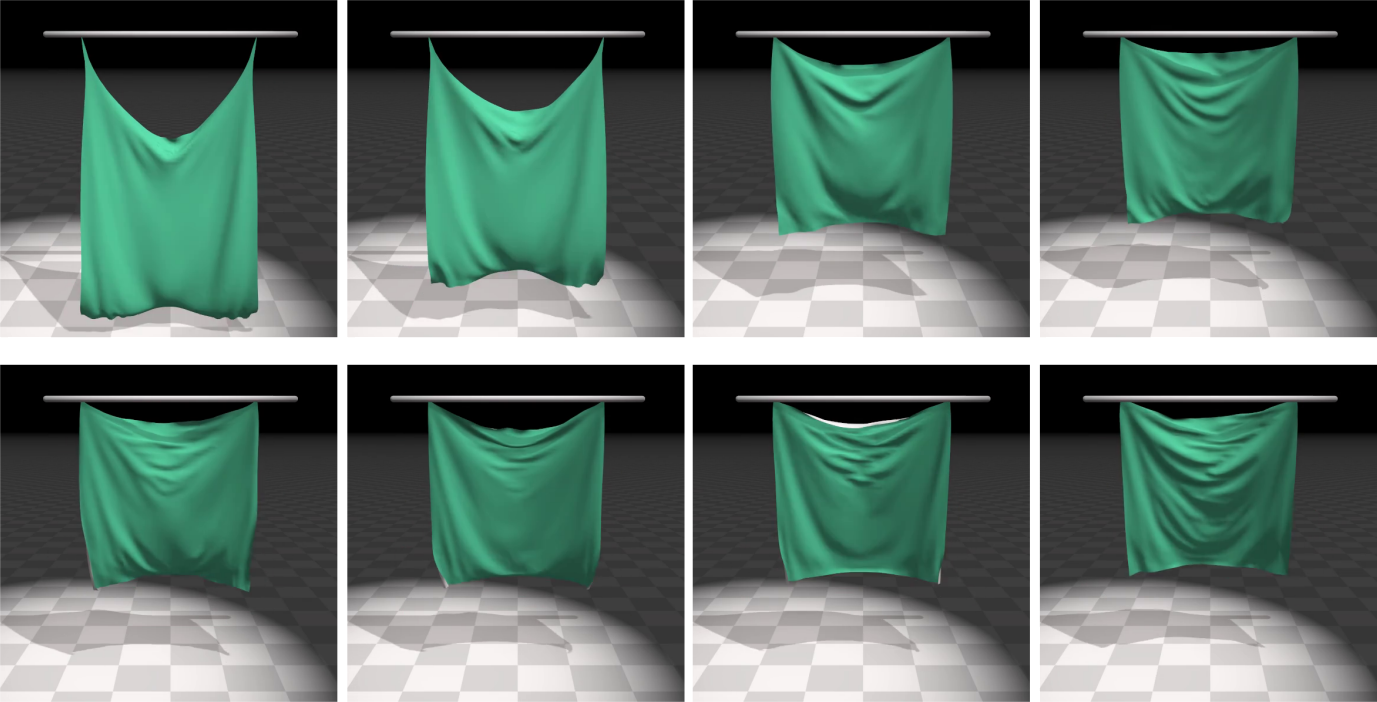
\includegraphics [scale=0.4] {my_folder/images//pbd_vs_xpbd}
	\caption{Сравнение работы алгоритмов PBD и XPBD на примере свисающей ткани спустя 20, 40, 80, 160 итераций (слева направо). Верхняя строка PBD, нижняя XPBD. Можно заметить, что растяжение ткани в алгоритме PBD нелинейно зависит от числа итераций, тогда как растяжение ткани при использовании алгоритма XPBD качественно неизменна }
	\label{fig:pbd-vs-xpbd}  
\end{figure}

	Соответствующий алгоритм $solveXPBDConstraint$ представлен на \firef{alg:SolveXPBDConstraint}

	\begin{algorithm} %[h]
		\SetKwFunction{solveXPBDConstraint}{} 
		\SetKwProg{myalg}{Algorithm}{}{}
		\nonl\myalg{solveXPBDConstraint}{
			\KwInput{
				время шага симуляции $\Delta t$,
				значения $\alpha$ и $\lambda$ для ограничения,
				размерность ограничения $n$,
				функция ограничения $C$, 
				текущие положения частиц $\{p_i\}_n$,
				обратные массы частиц $\{im_i\}_n$,
			}
			\KwOutput{вектора смещения частиц $\{\Delta p_i\}_n$ для удолветворения заданному ограничению, новое значение $\lambda$}
		
			$s = \frac{\alpha}{\Delta t^2}$;
		
			$scaleNum = -C(p_1, ...) - s \lambda$;
		
			$scaleDenum = \sum_{i}(im_i *|\nabla_{p_i} C(p_1, ..., p_{n})|^2) + s$;
		
			$scaleFactor = scaleNum/scaleDenum$;
		
			$\lambda = \lambda + scaleFactor$;
		
			\lFor {$i \in 1..n$}{
				$\Delta p_i = scaleFactor * im_i * \nabla_{p_i} C(p_1, ..., p_{n})$;
			}
		}
		\caption{Псевдокод алгоритма solveXPBDConstraint}
		\label{alg:SolveXPBDConstraint}
	\end{algorithm}
	\FloatBarrier
	
	Единственным недостатком данного алгоритма является то, что для его исполнения требуется дополнительная память для хранения параметров $\lambda$. Однако, вскоре авторами была выпущена ещё одна статья \cite{macklin2019small}, в которой ими было обнаружено, что вместо того, чтобы увеличивать количество итераций $solverIteration$, более эффективно запускать весь алгоритм несколько раз (обозначим это количество как $solverStep$), с уменьшенным промежутком времени. Таким образом, ими была предложена техника Small Steps, представленная на \firef{alg:ExtendedPositionBasedDynamicsSmallSteps}. При этом, крайний случай, при котором $solverIteration = 1$, не только является корректным и достаточно стабильным, но и позволяет избавится от доплнительных затрат памяти и процессорного времени на параметры $\lambda$, так как на первой итерации они равны 0.
	
	\begin{figure}[ht!] 
		\center
		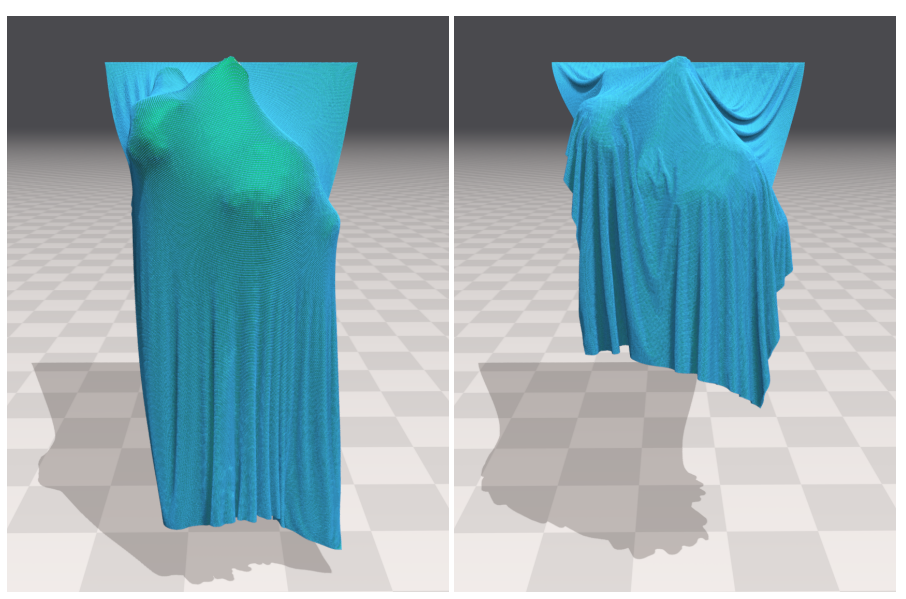
\includegraphics [scale=0.25] {my_folder/images//smallsteps}
		\caption{Сравнение XPBD с использованием техники Small Steps с различными параметрами. Слева $solverIteration = 30, solverStep = 1$, справа $solverIteration = 1, solverStep = 30$}.
		\label{fig:smallstep}  
	\end{figure}
	\FloatBarrier
		
	\begin{algorithm} %[h]
		\SetKwFunction{algoXPBDSmallStepsPseudocode}{} 
		\SetKwProg{myalg}{Algorithm}{}{} %write in 2nd agrument <<Algorithm>>, <<Procedure>> etc
		\nonl\myalg{\algoXPBDSmallStepsPseudocode}{
			\KwInput{
				время шага симуляции $\Delta t$,
				количество шагов $solverStep$,
				количество итераций $solverIteration$,
				текущее состояние частиц,
				предыдущее состояние частиц,
				ограничения,
				функция суммы внешних сил $f_{ext}(p)$
			}
			\KwOutput{положение частиц спустя заданное время $\{p_i(t + \Delta t)\}_N$}
			
			$st = \Delta t / solverStep$;
			
			\For{$step \in 1..solverStep$}{
				\lFor {$i \in 1..N$}{
					$v_i = \frac{p_i(t + (step - 1) * st) - p_i(t - (step - 2) * st)}{st} + st * im_i * f_{ext}(p_i)$
				}
			
				$dampVelocities(v_1, ... v_N)$;
			
				\lFor {$j \in 1..M $}{$\lambda_j = 0$}
			
				\lFor {$i \in 1..N $}{
					$p^*_i = p_i(t) + v_i * st$;
				}
				
				\lFor {$i \in 1..N $}{
					$genCollisionConstraints(p_i -> p^*_i)$;
				}
			
				\For{$k \in 1..solverIteration$}{
					$p^*_1, ..., p^*_N = projectXPBDConstraints(st, p^*_1, ..., p^*_N, \lambda_1, ..., \lambda_M)$;
				}
			
				\lFor {$i \in 1..N$}{
					$p_i(t + step * st) \leftarrow p^*_i$\
				}
			}
		}
		\caption{Псевдокод алгоритма Extended Position Based Dynamics с использованием техники Small Steps }\label{alg:ExtendedPositionBasedDynamicsSmallSteps}
	\end{algorithm}
	\FloatBarrier

%% Вспомогательные команды - Additional commands
%
%\newpage % принудительное начало с новой страницы, использовать только в конце раздела
%\clearpage % осуществляется пакетом <<placeins>> в пределах секций
%\newpage\leavevmode\thispagestyle{empty}\newpage % 100 % начало новой страницы